
\title{New figures from IBM analysis, final chapter}
\author{
        Chris McWilliams*, Alan Champneys, Miguel Lurgi,\\ Jose Montoya, Daniel Montoya \\ \\
				*Bristol Centre for Complexity Sciences, University of Bristol.\\
                chris.mcwilliams@bristol.ac.uk\\
}
\date{\today}

\documentclass[12pt]{article}
\usepackage{mathtools}
\usepackage{amsmath}
\usepackage{amssymb}
\usepackage{appendix}
\usepackage{graphicx}
\usepackage{caption}
\usepackage{subcaption}
\usepackage{rotating}
%\usepackage{subfig}
\usepackage[font={small,it}]{caption}
\usepackage[font={small,it}]{subcaption}
\usepackage{todo}
\setlength\parindent{0pt}
\setlength{\parskip}{10pt plus 1pt minus 1pt}

\newcommand{\mbeq}{\overset{!}{=}}

\begin{document}
NOTE paper: Coevolution can reverse predator–prey cycles
In the previous analysis we have characterised the performance of the \emph{gradient-matching} (GM) method at fitting the GLV model to population dynamics simulated using the IBM. The analysis has highlighted the following issues:
\begin{itemize}
	\item The method does not \emph{consistently} identify the true interaction network topology
	\item When fitting the GLV with the topology restricted to match the true topology, the fit does not necessarily outperform competing models (with alternative topologies) in terms of:
		\begin{itemize}
			\item The value of the error function
			\item The location of the equilibrium
			\item The local stability of the equilibrium
			\item The estimated rates of biomass flow between species.
		\end{itemize}		   
\end{itemize}
In general we have shown that the performance of the method, regarding the issues listed above, deteriorates both as the number of species is increased, and as the immigration rate (IR) is increased. Neither result is surprising since increasing the number of species combinatorially increases the number of potential topologies, and increasing the IR increases the stochastic component of the dynamics (as we saw in chapter \ref{chap:WHERE}). The main failure of the method in identification of the true interaction network topology is that it often detects strong spurious interactions between species which share no direct link in the network. The detection of spurious interactions is a problem that has plagued previous attempts to infer interactions between species [CITATIONS]. In our case the detection of apparently spurious \emph{competitive} interactions may be informative, since we have previously seen evidence of strong competition effects in the IBM (chapters \ref{} and \ref{}). However the most frequent spurious interaction detected has proven to be an \emph{antagonism} between basal and top predator species. Moreover the direction of the detected link implies that the \emph{plant eats the top-predator}. This is clearly wrong. In what follows we attempt to explain the propensity of the GM method to produce such erroneous conclusions. 

\begin{figure}
	\centering
	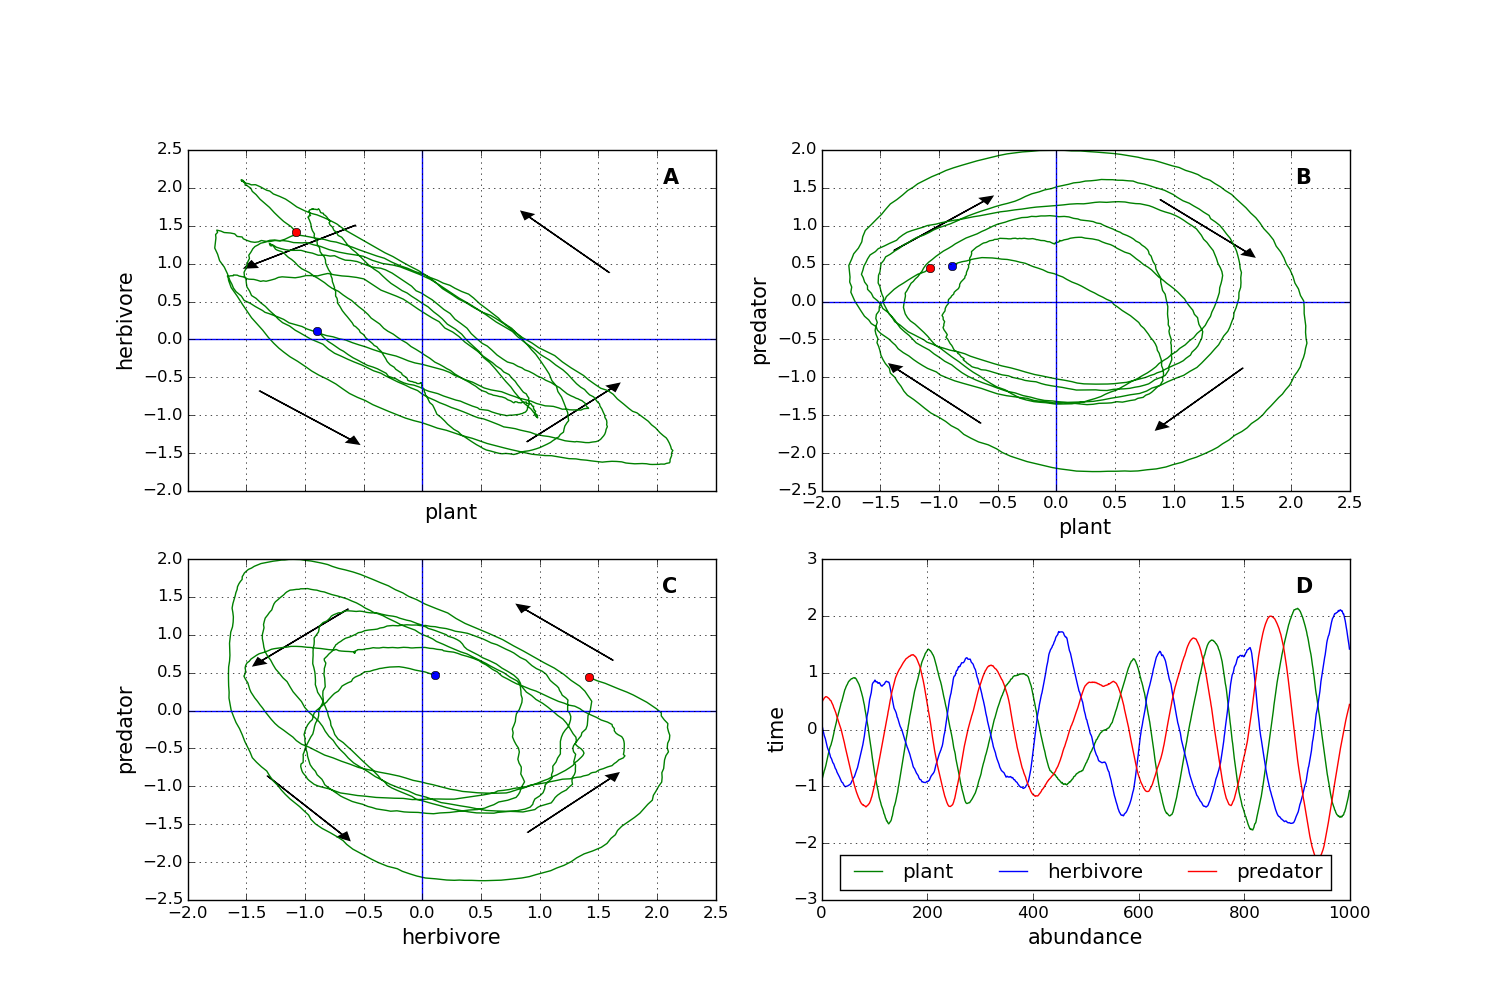
\includegraphics[width=\textwidth]{{{3species/3sp_phase_plane}}}
	\caption{Example of three species IBM dynamics for a food chain. Panels A-C: phase plane projections of trajectory for pairs of species. Plane is split into four quadrants centred on mean species abundances. Arrows indicate average direction (unit) vector of trajectory in each quadrant. Blue and red dots indicate start and finish of trajectory respectively. Panel D: Corresponding population dynamic time series for all three species.}
	\label{fig:3sp_phase_plane}
\end{figure}

For simplicity we focus on the case of a three-species food chain. However the following argument generalises to larger numbers of species. In classical predator-prey models, without time-delay or other embellishments, there is a phase-lag between the prey and the predator population. That is, the peak in prey abundance \emph{precedes} the peak in predator abundance. Some previous attempts to infer species interactions have done so by characterising the relative phases in species oscillations [CITATIONS]. Similar to the approach of Sandvik et al. we look at the phase relationships between the species in our three species food-chain. Figure \ref{fig:3sp_phase_plane} (panels A-C) shows the projection of the three species population dynamics projected onto the phase plane defined by each pair of species. In each case the species in the lower trophic level is plotted on the x-axis, such that a classical predator-prey interaction should generate counter-clockwise rotation. Panels A and C shows pairs of species which \emph{do interact} in the model, and indeed the observed rotation is counter-clockwise. Panel B shows the phase plane defined by the plant and the top-predator species, which do not interact in the model. In this case there is a clear clockwise rotation in the phase plane. The phase relationship suggests that the predator eats the plant, although there is no such interaction in the model. From the time series dynamics, plotted in panel D, it is clear that the phase relationship results from robust oscillations produced by the other two interactions. Here lies the problem with the method. In a complex community phase relationships may emerge which are suggestive of an interaction. Since the GM method estimates the parameters for each species independently it is free to conclude that such suggested interactions are \emph{real} without concern for the consequences of such interactions in the fully coupled system\footnote{This needs to be made rigorous.}.

Figure \ref{fig:3sp_fourier_corr} shows how Fourier analysis analysis and cross-correlation can be used to calculate the phase relationship between two species..(I saw something similar in a blog post, but not in a publication. I think it is OK?)

\begin{figure}
	\centering
	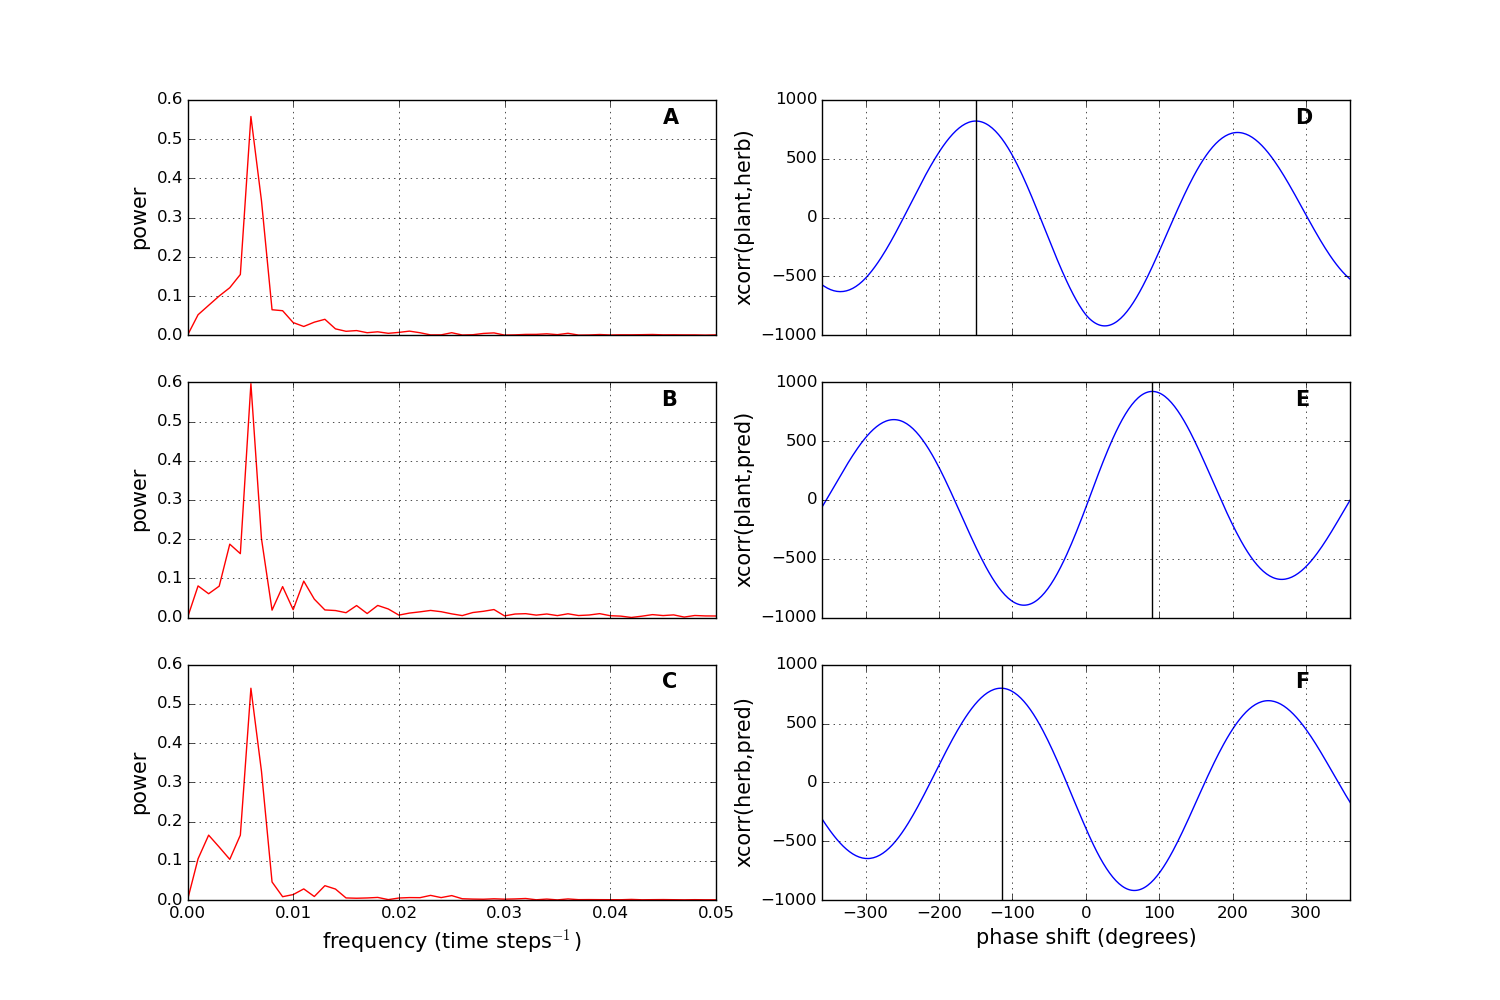
\includegraphics[width=\textwidth]{{{3species/3sp_fourier_corr}}}
	\caption{Fourier analysis of the dynamics shown in figure \ref{fig:3sp_phase_plane}. Panels A,B,C: Fourier frequency spectrum for the plant, herbivore and predator time series respectively. Panels D,E,F: Cross-correlation (xcorr) between the three time-series, as labelled in the figure and corresponding to the phase portraits in figure \ref{fig:3sp_phase_plane}, panels A,B,C. Phase shift is given in degree relative to the dominant time period of the first time series in the cross-correlation, determined from the Fourier spectrum. Black vertical lines indicate location of maximum correlation.}
	\label{fig:3sp_fourier_corr}
\end{figure}
\section{2 species, no habitat loss.}

These figures show results from fitting GLV model to 2 species IBM simulations.

\begin{figure}[b]
	\centering
	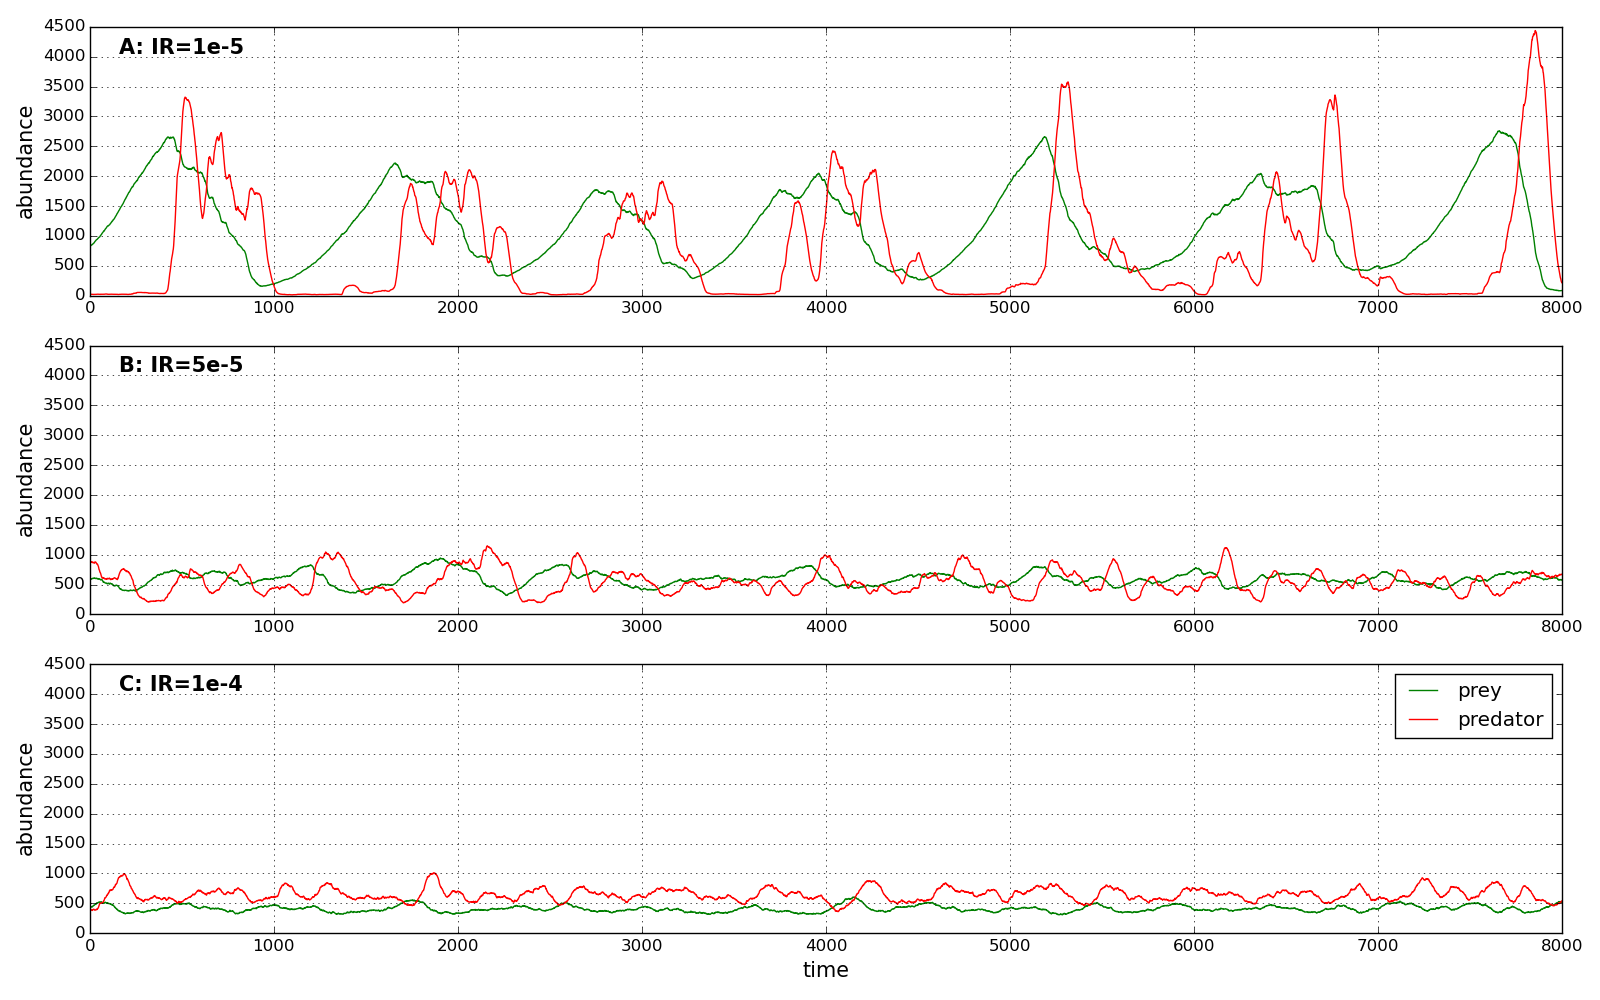
\includegraphics[width=\textwidth]{{{2species/old/example_dynamics_2sp_nohl}}}
	\label{fig:example_dynamics}
	\caption{Example dynamics of three simulation runs with different IR. Initial transience removed.}
\end{figure}

\begin{figure}[b]
	\centering
	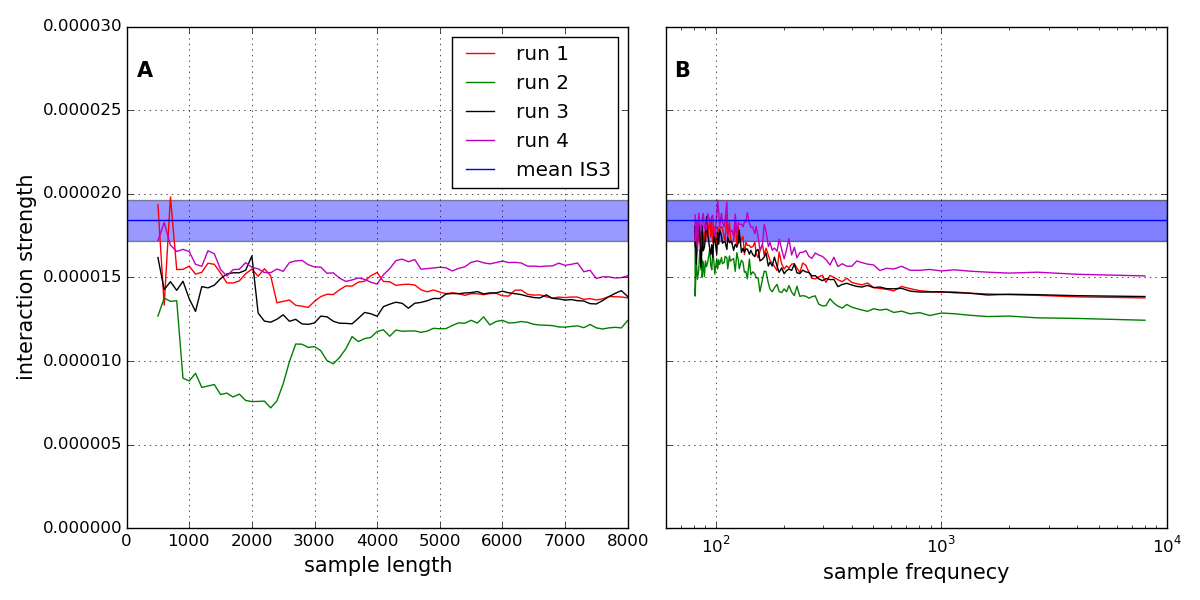
\includegraphics[width=\textwidth]{{{2species/old/convergence_highIR}}}
	\label{fig:conv_high}
	\caption{Convergence of estimator $\hat{J}_{01}$. High IR (0.0001).}
\end{figure}

\begin{figure}
	\centering
	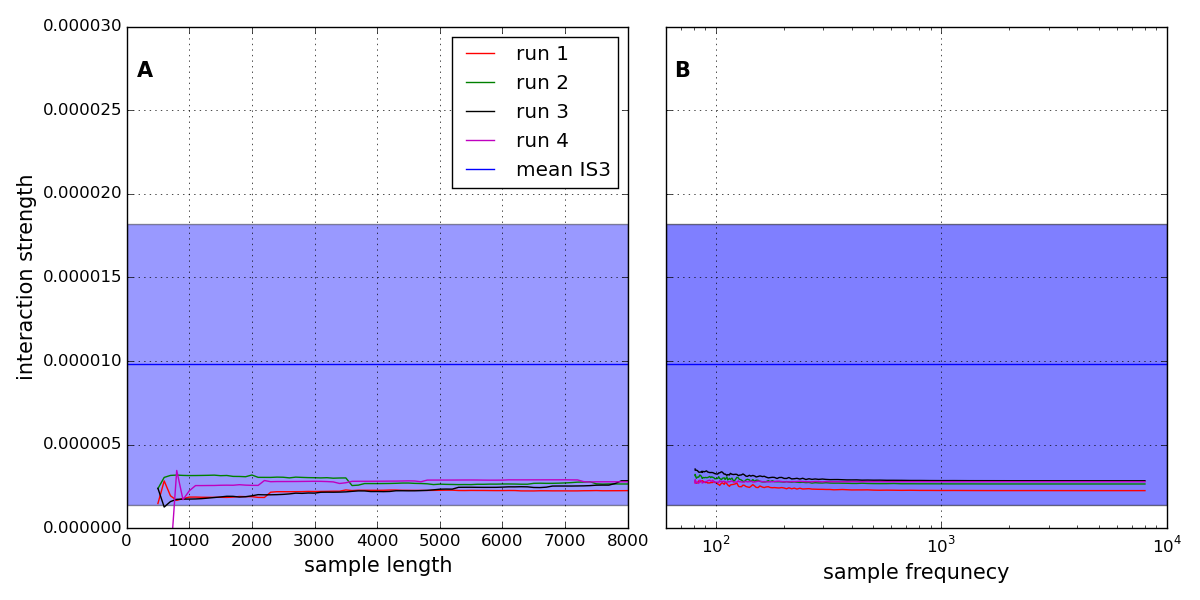
\includegraphics[width=\textwidth]{{{2species/old/convergence_lowIR}}}
	\label{fig:conv_low}
	\caption{Convergence of estimator $\hat{J}_{01}$. Low IR (0.00001).}
\end{figure}


\begin{figure}
	\centering
	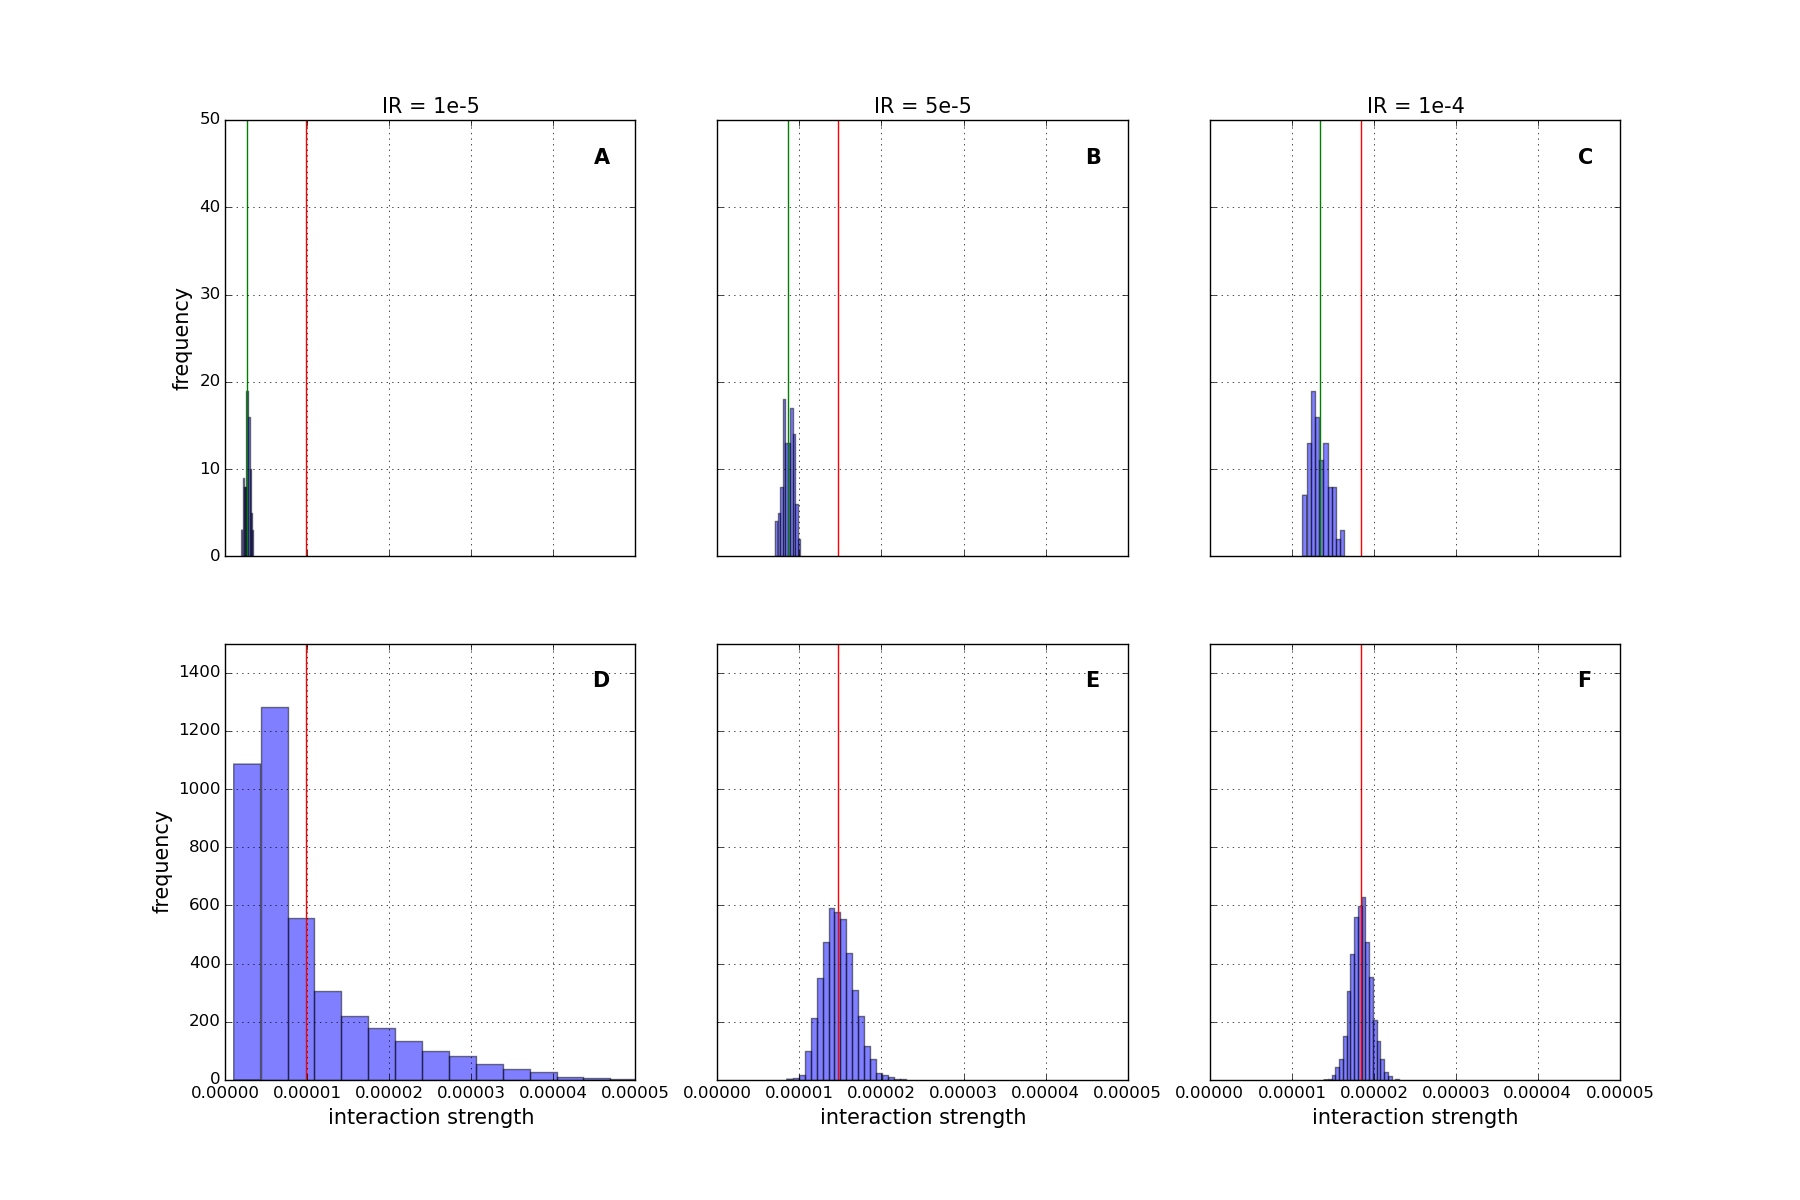
\includegraphics[width=\textwidth]{{{2species/old/J01_ensemble_estimates_2sp_nohl}}}
	\label{fig:ensemble_J01}
	\caption{Distribution of prey interaction strengths for three ensembles of simulations at different IR. Top row: estimates produced by fitting GLV model. Bottom row: Estimates produced by counting number of prey consumed.}
\end{figure}


\begin{figure}
	\centering
	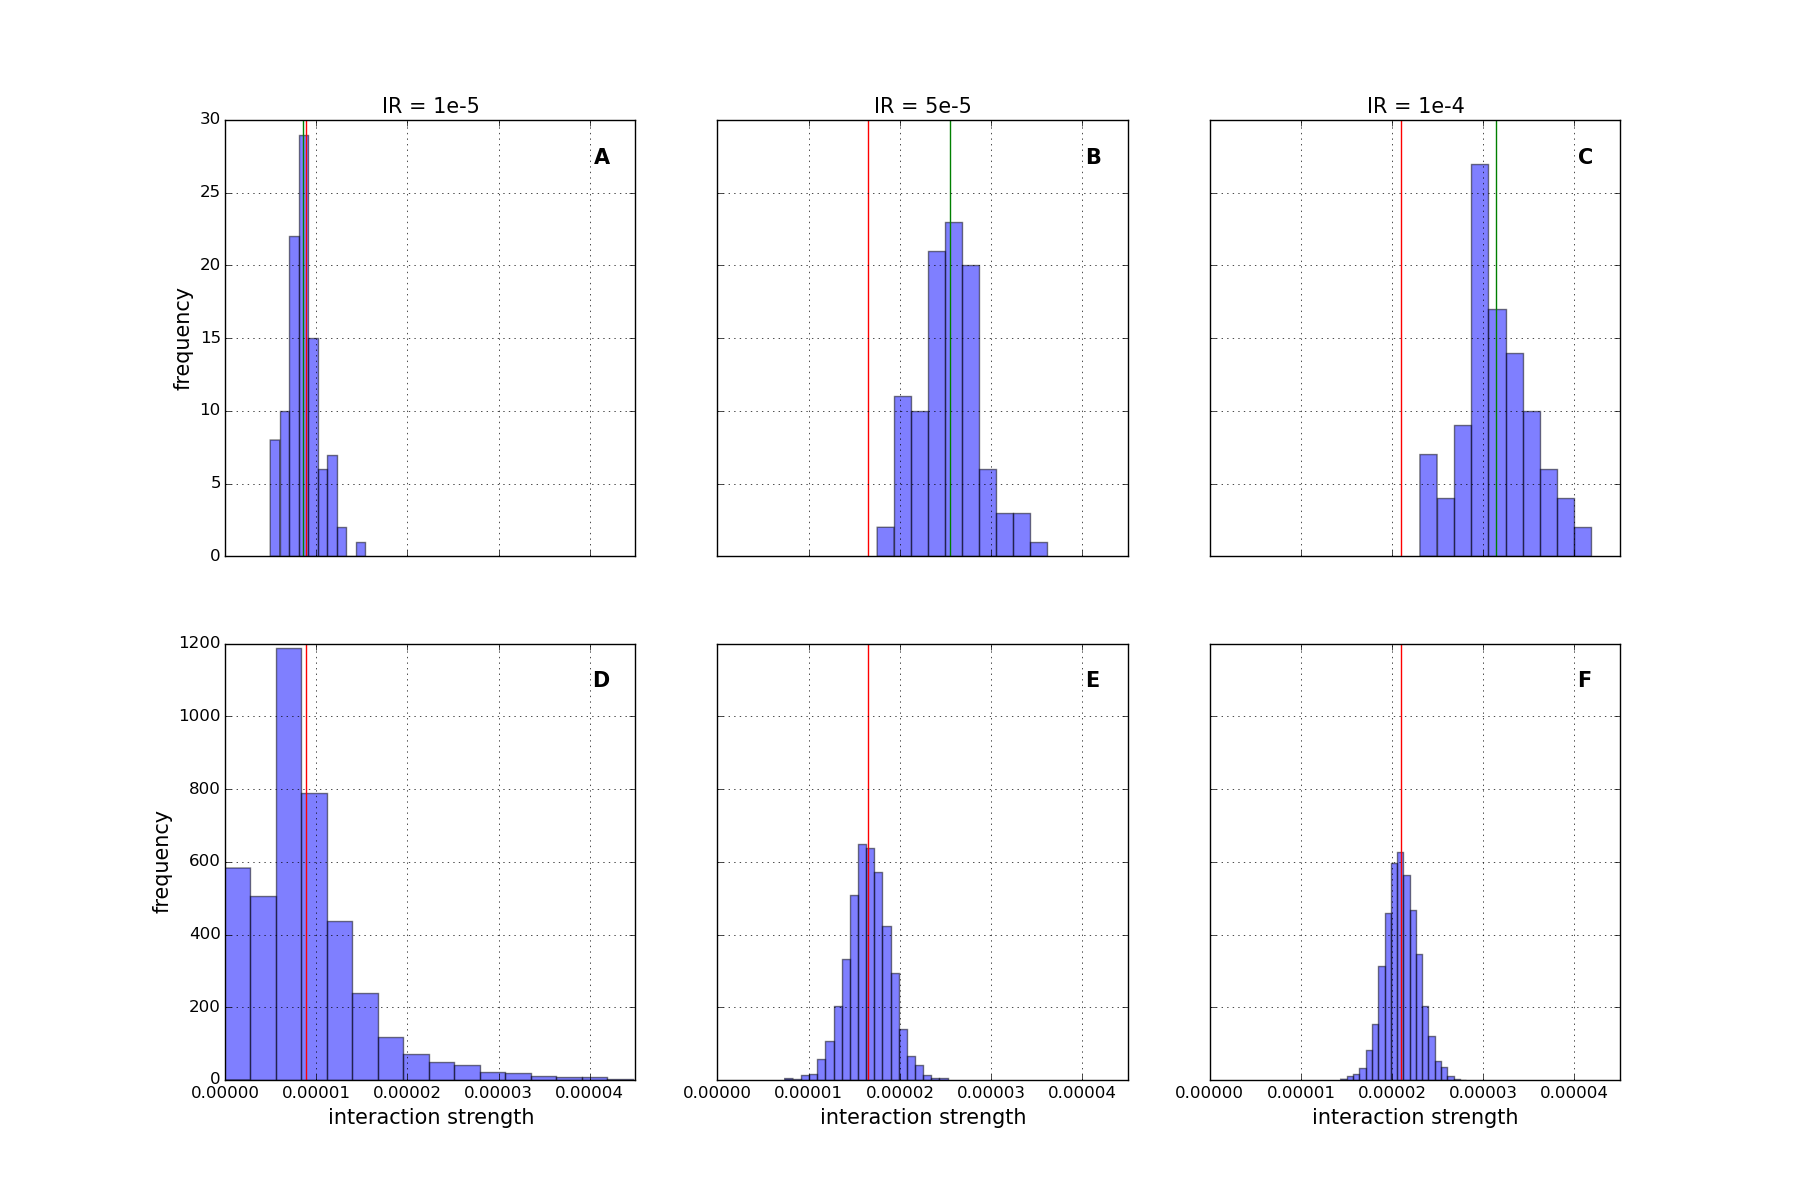
\includegraphics[width=\textwidth]{{{2species/old/J10_ensemble_estimates_2sp_nohl}}}
	\label{fig:ensemble_J10}
	\caption{Distribution of predator interaction strengths for three ensembles of simulations at different IR. Top row: estimates produced by fitting GLV model. Bottom row: Estimates produced by counting number of predators born.}
\end{figure}


\begin{figure}
	\centering
	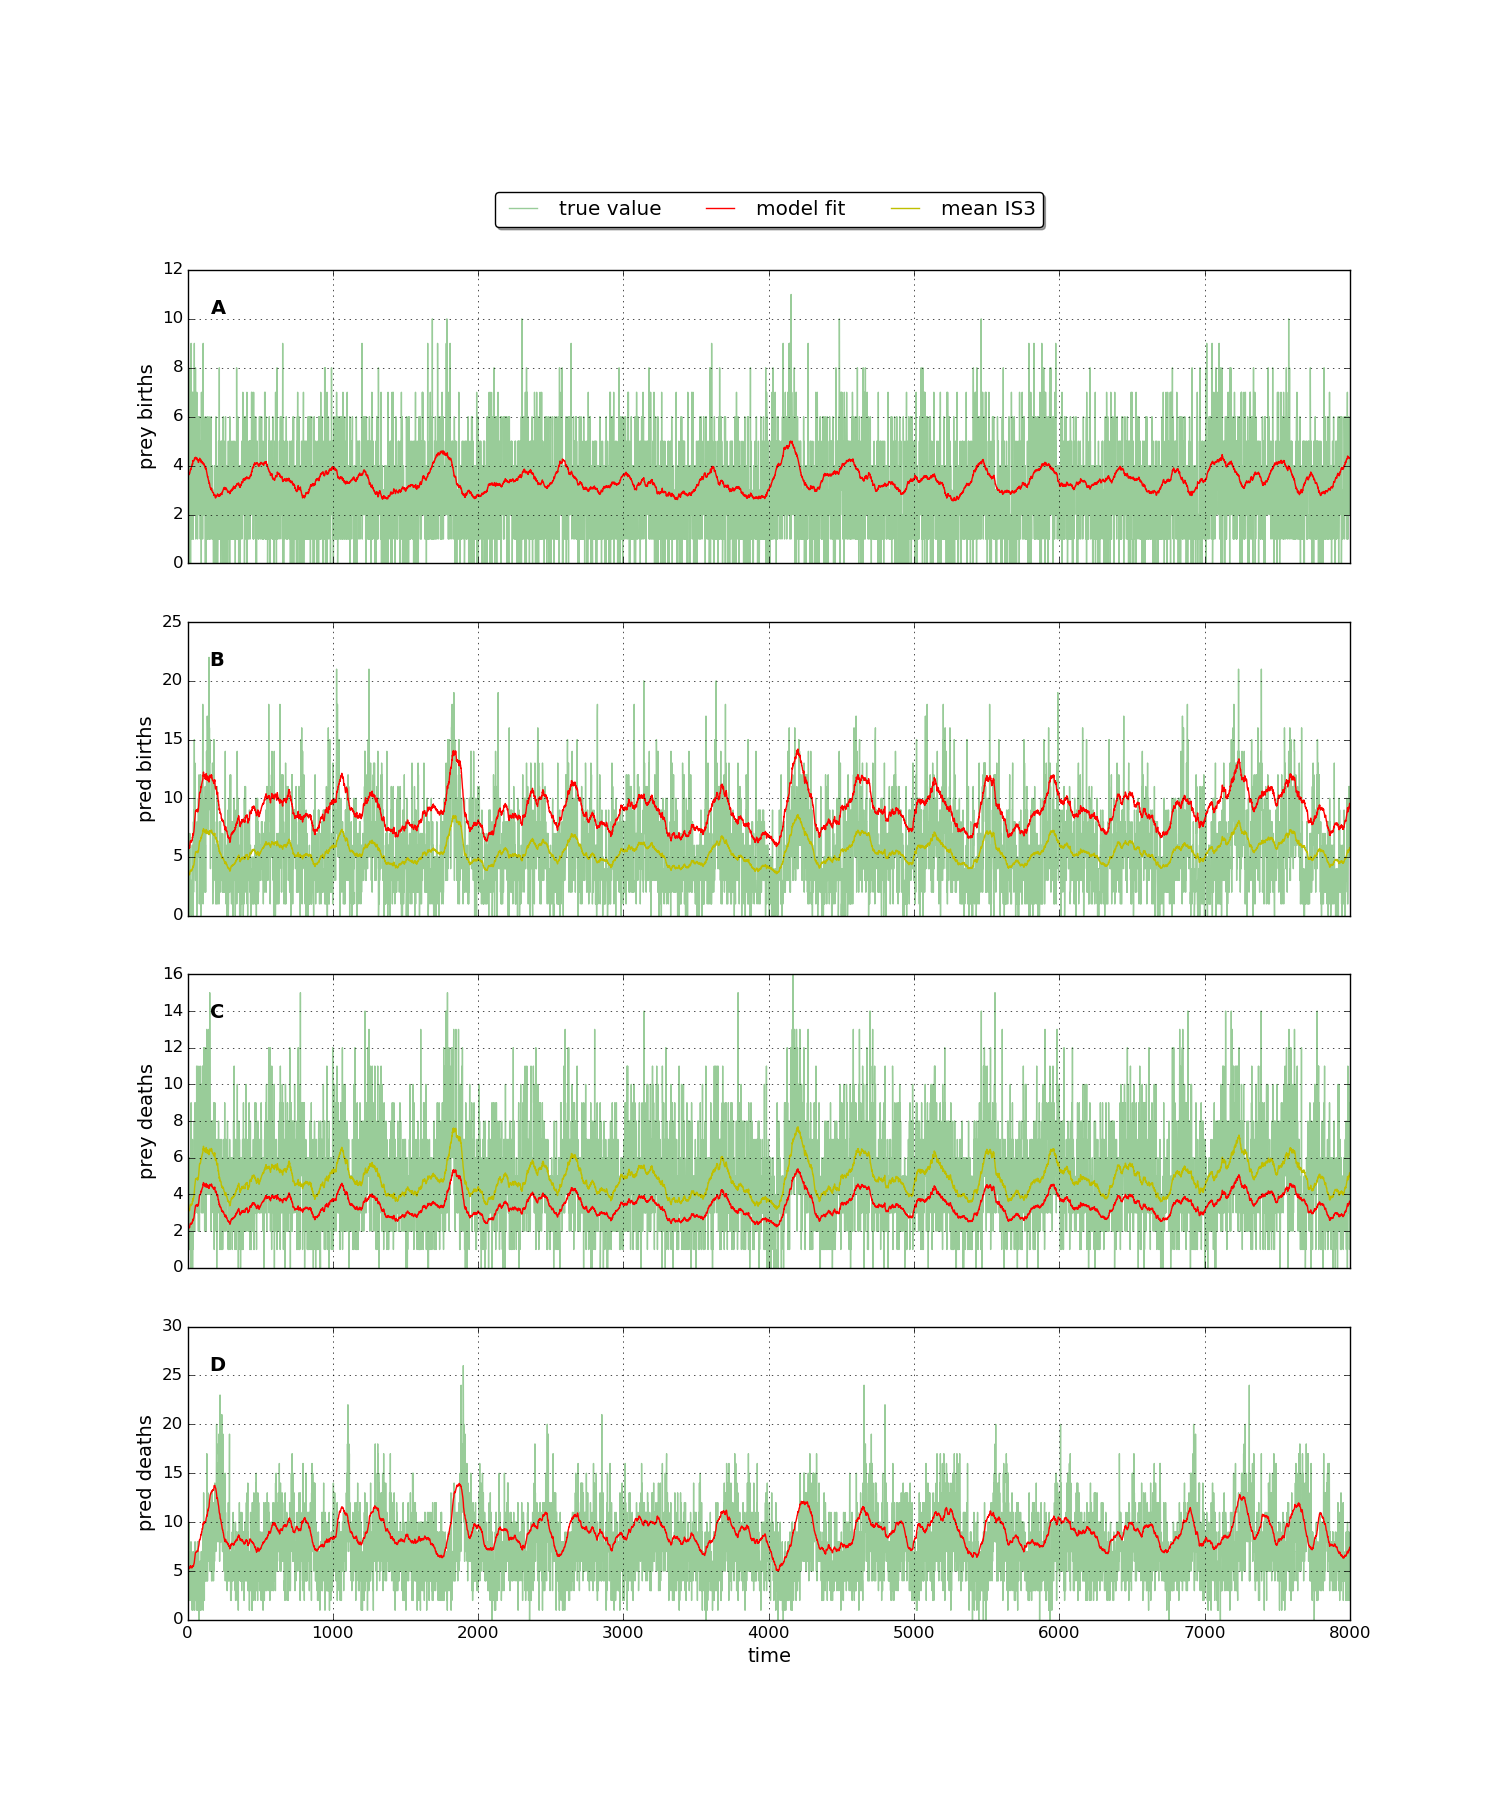
\includegraphics[width=\textwidth]{{{2species/old/back_check_highIR_4463199_4}}}
	\label{fig:backcheck_high}
	\caption{Comparing actual births and death rates to those predicted by the fitted model. Single simulation run, high IR (0.0001)}
\end{figure}


\begin{figure}
	\centering
	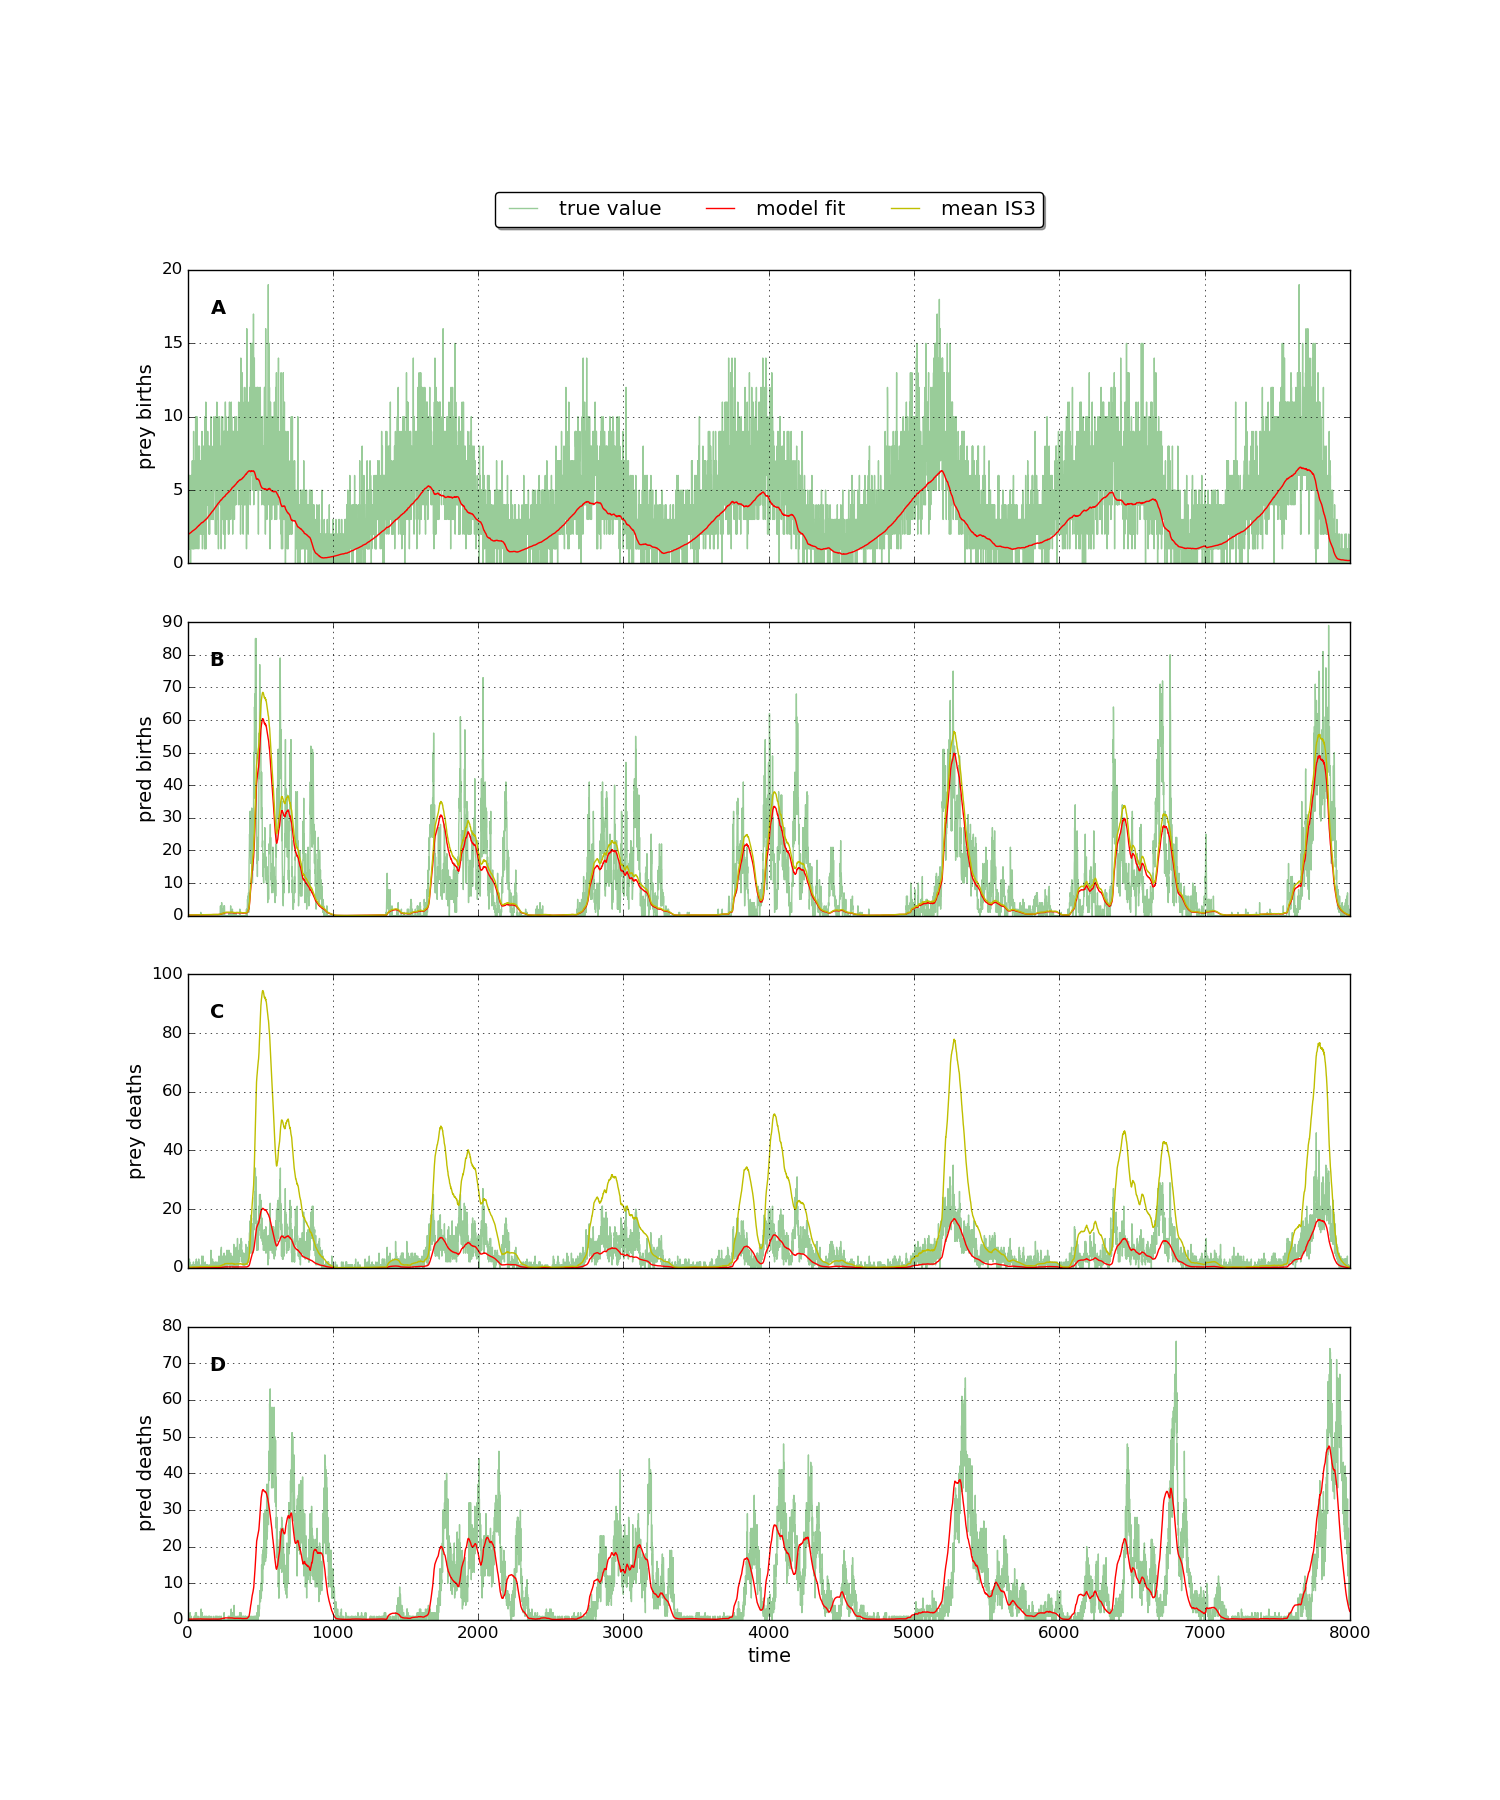
\includegraphics[width=\textwidth]{{{2species/old/back_check_lowIR_4463195_3}}}
	\label{fig:backcheck_low}
	\caption{Comparing actual births and death rates to those predicted by the fitted model. Single simulation run, low IR (0.00001)}
\end{figure}


\clearpage
\section{2 species, with habitat loss.}

\begin{figure}[b]
	\centering
	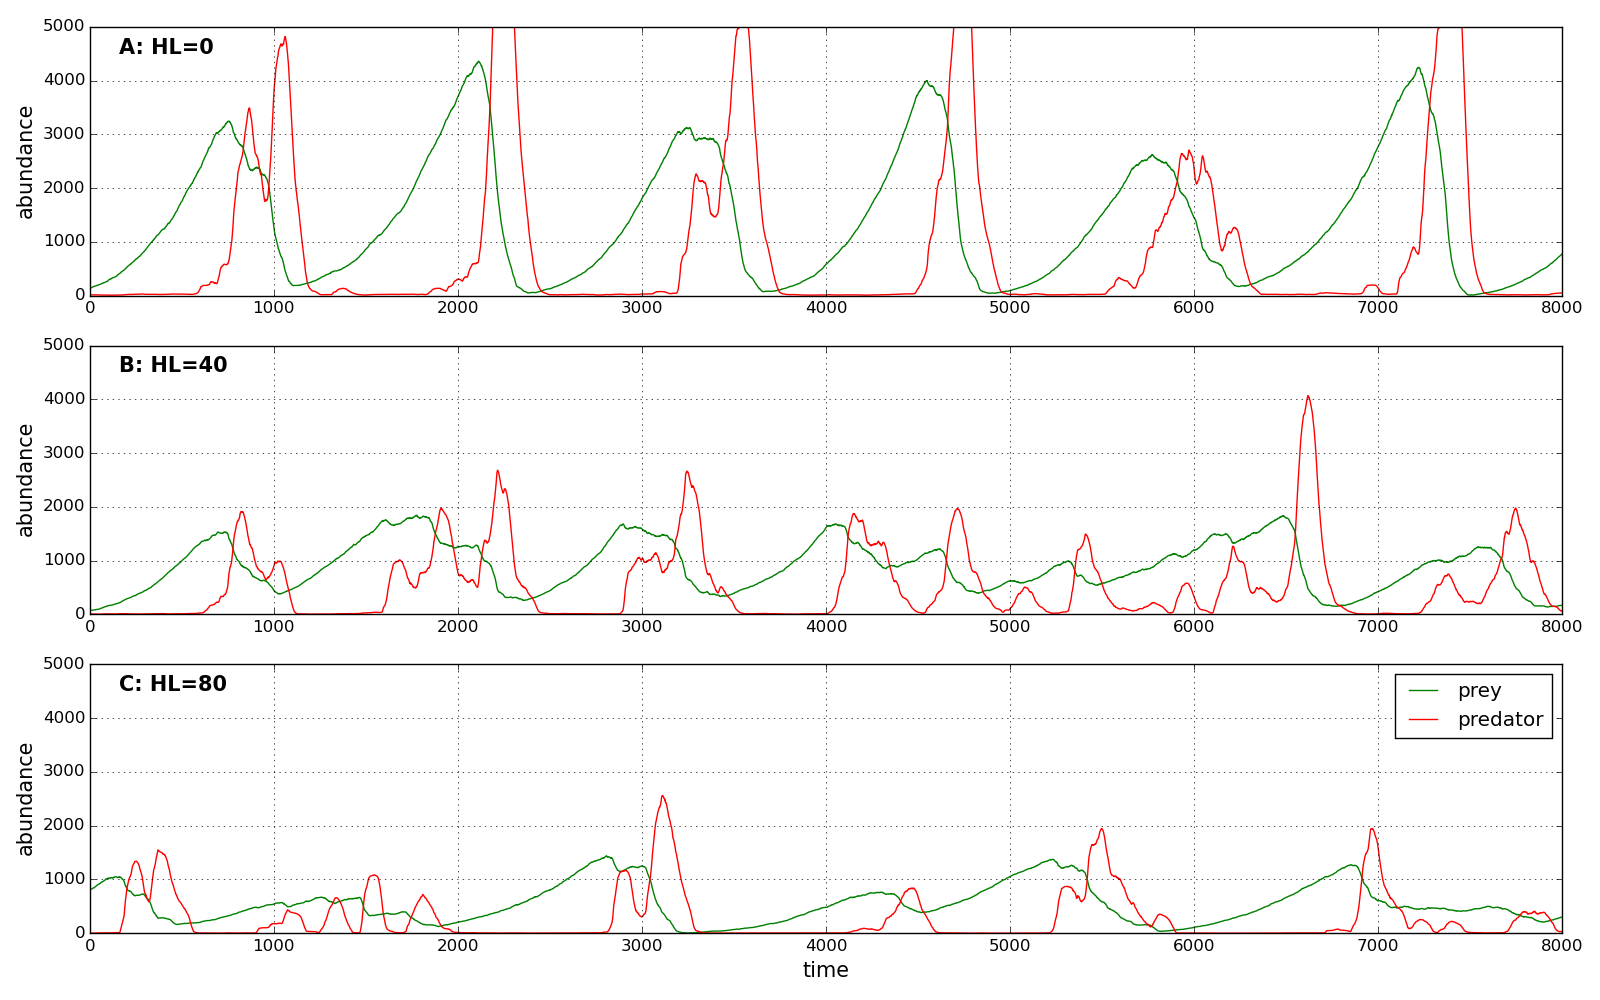
\includegraphics[width=\textwidth]{{{2species/old/example_dynamics_2sp_contiguous}}}
	\label{fig:example_dynamics_contig}
	\caption{Example dynamics of three simulation runs with different levels of contiguous HL. Initial transience removed.}
\end{figure}

\begin{figure}[b]
	\centering
	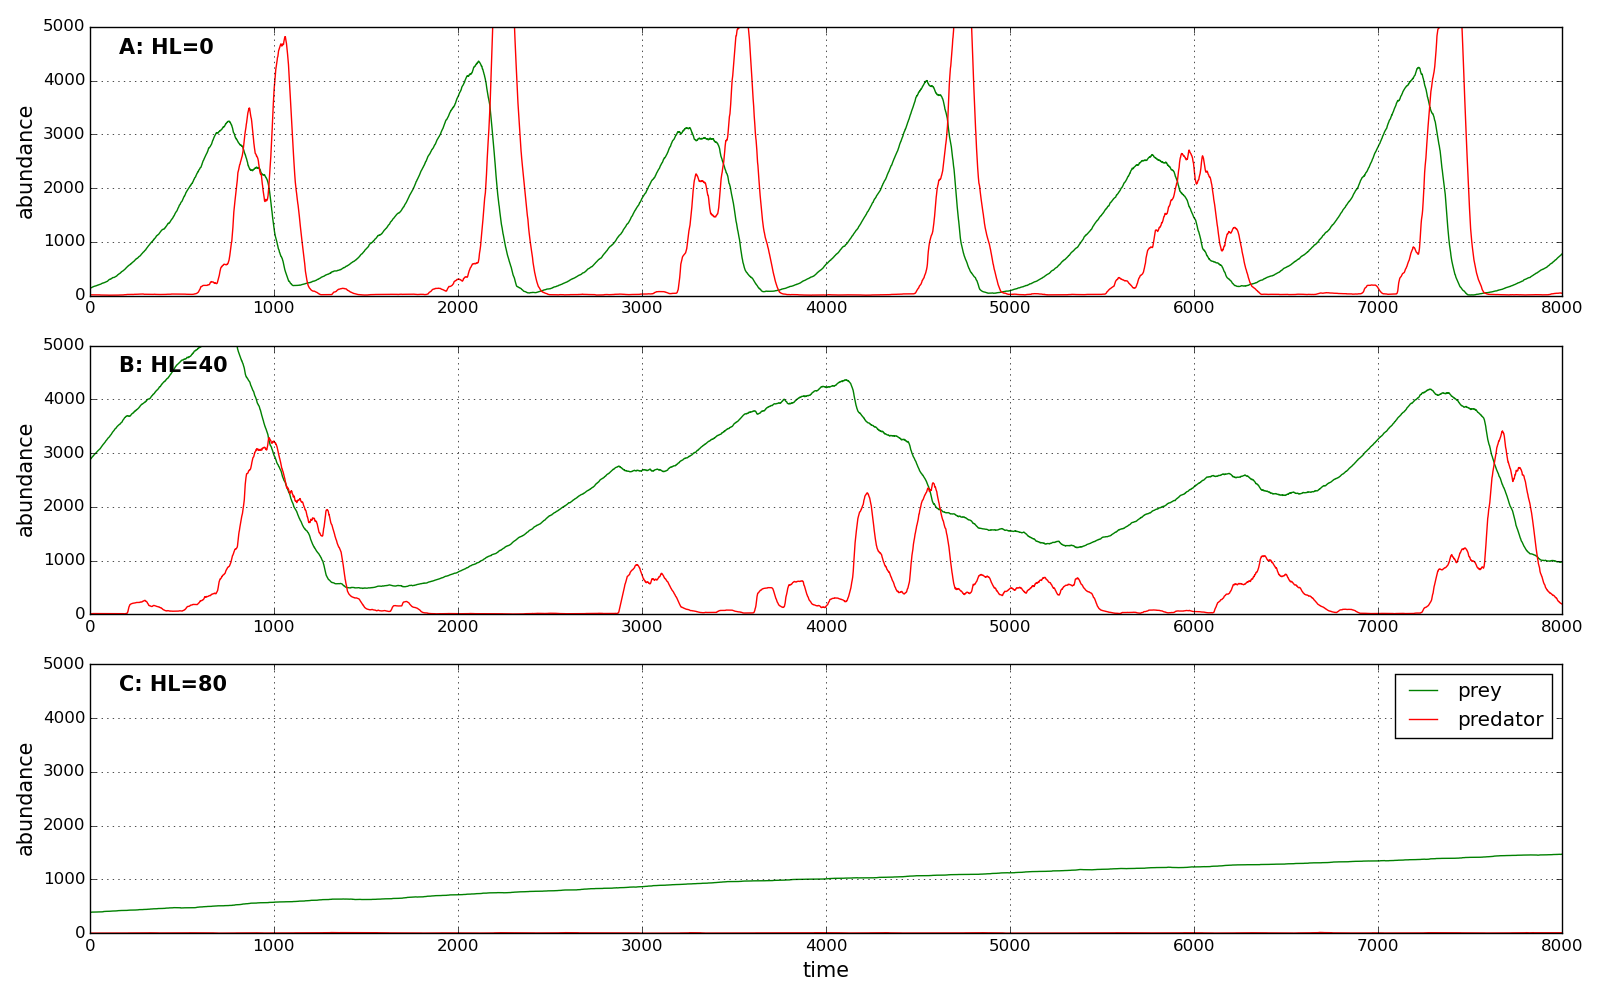
\includegraphics[width=\textwidth]{{{2species/old/example_dynamics_2sp_random}}}
	\label{fig:example_dynamics_rand}
	\caption{Example dynamics of three simulation runs with different levels of random HL. Initial transience removed.}
	\end{figure}



\end{document}


